\documentclass[border=4pt,tikz]{standalone}
\usepackage[T1]{fontenc}
\usepackage{lmodern}
\usetikzlibrary{positioning,arrows.meta,calc,fit,backgrounds,patterns}
% Shared visual language for the paper's architecture diagrams.
% Every fill differs in lightness, so the diagrams stay legible when printed
% in grayscale; colour is only a redundant cue.
\definecolor{ink}{HTML}{1B2A3A}
\definecolor{navyfill}{HTML}{D5E0EC}
\definecolor{navyedge}{HTML}{2F5D8A}
\definecolor{tealfill}{HTML}{BFD8D5}
\definecolor{tealedge}{HTML}{2A6F6C}
\definecolor{amberfill}{HTML}{F1DCAE}
\definecolor{amberedge}{HTML}{9C6512}
\definecolor{greyfill}{HTML}{E5E7EB}
\definecolor{greymid}{HTML}{8B939E}
\definecolor{redfill}{HTML}{F0CBC5}
\definecolor{rededge}{HTML}{9E3B32}

\tikzset{
  >={Stealth[length=2.0mm,width=1.5mm]},
  every node/.style={font=\footnotesize, text=ink},
  box/.style={draw=ink, line width=0.5pt, rounded corners=1.5pt,
              fill=greyfill, align=center, inner sep=3pt, minimum height=7mm},
  databox/.style={box, fill=amberfill, draw=amberedge},
  procbox/.style={box, fill=navyfill, draw=navyedge},
  repbox/.style={box, fill=tealfill, draw=tealedge},
  evalbox/.style={box, fill=redfill, draw=rededge},
  fadebox/.style={box, fill=white, draw=greymid, dashed},
  arr/.style={->, draw=ink, line width=0.6pt},
  darr/.style={->, draw=greymid, line width=0.6pt, dashed},
  lbl/.style={font=\scriptsize, text=ink, inner sep=1pt, fill=white, fill opacity=0.85, text opacity=1},
  note/.style={font=\scriptsize, text=ink, align=left, inner sep=1pt},
  badge/.style={draw=rededge, fill=redfill, rounded corners=6pt,
                font=\scriptsize\bfseries, text=rededge, inner sep=2.2pt},
  badgefrz/.style={draw=tealedge, fill=tealfill, rounded corners=6pt,
                font=\scriptsize\bfseries, text=tealedge, inner sep=2.2pt},
  group/.style={draw=greymid, line width=0.5pt, rounded corners=3pt, inner sep=6pt},
}


% Shapes are taken from results/model_arch.json (measured with forward hooks on
% the actual vggface2 checkpoint, batch dimension dropped). Naming follows
% facenet-pytorch 2.5.3, not the published Inception-ResNet figure.
\begin{document}
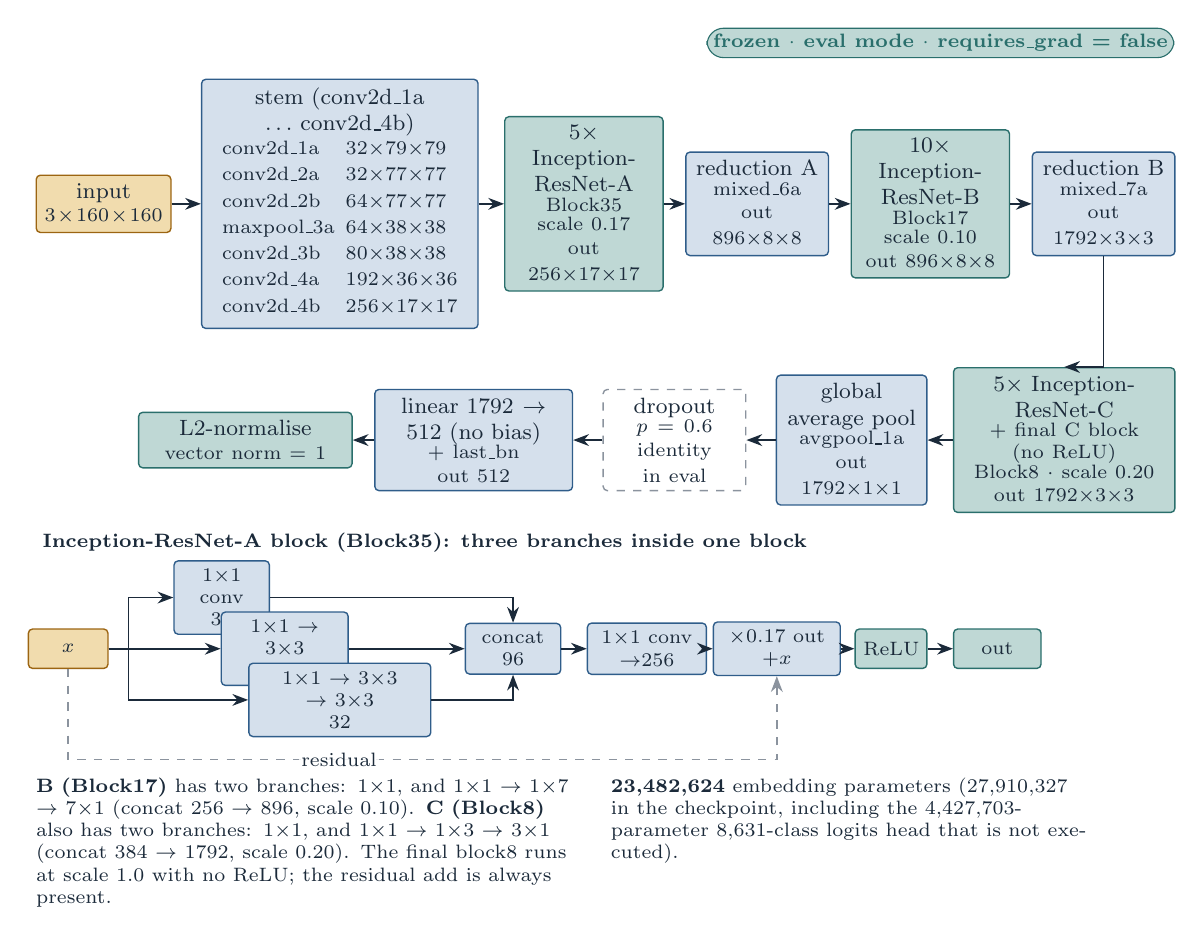
\begin{tikzpicture}[x=1cm,y=1cm]

% ------------------------------------------------------------------ row 1
\node[databox, text width=1.5cm] (input) at (1.00,3.20)
  {input\\[-1pt] \scriptsize $3\times160\times160$};

\node[procbox, text width=3.3cm] (stem) at (4.00,3.20)
  {stem (conv2d\_1a $\ldots$ conv2d\_4b)\\[-1pt]
   \begin{tabular}{@{}l@{\hspace{4pt}}l@{}}
     \scriptsize conv2d\_1a & \scriptsize $32{\times}79{\times}79$\\
     \scriptsize conv2d\_2a & \scriptsize $32{\times}77{\times}77$\\
     \scriptsize conv2d\_2b & \scriptsize $64{\times}77{\times}77$\\
     \scriptsize maxpool\_3a & \scriptsize $64{\times}38{\times}38$\\
     \scriptsize conv2d\_3b & \scriptsize $80{\times}38{\times}38$\\
     \scriptsize conv2d\_4a & \scriptsize $192{\times}36{\times}36$\\
     \scriptsize conv2d\_4b & \scriptsize $256{\times}17{\times}17$
   \end{tabular}};

\node[repbox, text width=1.8cm] (a) at (7.10,3.20)
  {5$\times$ Inception-ResNet-A\\[-1pt] \scriptsize Block35\\[-1pt] \scriptsize scale 0.17\\[-1pt] \scriptsize out $256{\times}17{\times}17$};
\node[procbox, text width=1.6cm] (redA) at (9.30,3.20)
  {reduction A\\[-1pt] \scriptsize mixed\_6a\\[-1pt] \scriptsize out $896{\times}8{\times}8$};
\node[repbox, text width=1.8cm] (b) at (11.50,3.20)
  {10$\times$ Inception-ResNet-B\\[-1pt] \scriptsize Block17\\[-1pt] \scriptsize scale 0.10\\[-1pt] \scriptsize out $896{\times}8{\times}8$};
\node[procbox, text width=1.6cm] (redB) at (13.70,3.20)
  {reduction B\\[-1pt] \scriptsize mixed\_7a\\[-1pt] \scriptsize out $1792{\times}3{\times}3$};

\draw[arr] (input) -- (stem);
\draw[arr] (stem) -- (a);
\draw[arr] (a) -- (redA);
\draw[arr] (redA) -- (b);
\draw[arr] (b) -- (redB);

% ------------------------------------------------------------------ row 2 (flow right to left)
\node[repbox, text width=2.6cm] (c) at (13.20,0.20)
  {5$\times$ Inception-ResNet-C\\[-1pt] \scriptsize + final C block (no ReLU)\\[-1pt] \scriptsize Block8 $\cdot$ scale 0.20\\[-1pt] \scriptsize out $1792{\times}3{\times}3$};
\node[procbox, text width=1.7cm] (gap) at (10.50,0.20)
  {global average pool\\[-1pt] \scriptsize avgpool\_1a\\[-1pt] \scriptsize out $1792{\times}1{\times}1$};
\node[fadebox, text width=1.6cm] (drop) at (8.25,0.20)
  {dropout\\[-1pt] \scriptsize $p=0.6$\\[-1pt] \scriptsize identity in eval};
\node[procbox, text width=2.3cm] (lin) at (5.70,0.20)
  {linear $1792\to512$ (no bias)\\[-1pt] \scriptsize + last\_bn\\[-1pt] \scriptsize out 512};
\node[repbox, text width=2.5cm] (out) at (2.80,0.20)
  {L2-normalise\\[-1pt] \scriptsize vector norm $=1$};

\draw[arr] (redB.south) -- (redB.south |- c.north) -- (c.north);
\draw[arr] (c) -- (gap);
\draw[arr] (gap) -- (drop);
\draw[arr] (drop) -- (lin);
\draw[arr] (lin) -- (out);

% ------------------------------------------------------------------ block inset
\node[font=\scriptsize\bfseries, anchor=south west] at (0.10,-1.35)
  {Inception-ResNet-A block (Block35): three branches inside one block};
\node[databox, text width=0.8cm, minimum height=5mm, font=\scriptsize] (xin) at (0.55,-2.45) {$x$};
\node[procbox, text width=1.0cm, minimum height=5mm, font=\scriptsize] (br0) at (2.50,-1.80) {1$\times$1 conv\\32};
\node[procbox, text width=1.4cm, minimum height=5mm, font=\scriptsize] (br1) at (3.30,-2.45) {1$\times$1 $\to$ 3$\times$3\\32};
\node[procbox, text width=2.1cm, minimum height=5mm, font=\scriptsize] (br2) at (4.00,-3.10) {1$\times$1 $\to$ 3$\times$3 $\to$ 3$\times$3\\32};
\node[procbox, text width=1.0cm, minimum height=5mm, font=\scriptsize] (cat) at (6.20,-2.45) {concat\\96};
\node[procbox, text width=1.3cm, minimum height=5mm, font=\scriptsize] (proj) at (7.90,-2.45) {1$\times$1 conv\\$\to$256};
\node[procbox, text width=1.4cm, minimum height=5mm, font=\scriptsize] (add) at (9.55,-2.45) {$\times0.17$ out\\$+x$};
\node[repbox, text width=0.7cm, minimum height=5mm, font=\scriptsize] (relu) at (11.00,-2.45) {ReLU};
\node[repbox, text width=0.9cm, minimum height=5mm, font=\scriptsize] (xout) at (12.35,-2.45) {out};

\draw[arr] (xin.east) -- ++(0.25,0) |- (br0.west);
\draw[arr] (xin.east) -- ++(0.25,0) |- (br1.west);
\draw[arr] (xin.east) -- ++(0.25,0) |- (br2.west);
\draw[arr] (br0.east) -| (cat.north);
\draw[arr] (br1.east) -- (cat.west);
\draw[arr] (br2.east) -| (cat.south);
\draw[arr] (cat) -- (proj);
\draw[arr] (proj) -- (add);
\draw[arr] (add) -- (relu);
\draw[arr] (relu) -- (xout);
\draw[darr] (xin.south) -- ++(0,-1.15) -| node[lbl, right=1pt, pos=0.16] {residual} (add.south);

\node[note, anchor=north west, text width=6.9cm] at (0.10,-4.05)
  {\textbf{B (Block17)} has two branches: 1$\times$1, and 1$\times$1 $\to$ 1$\times$7 $\to$ 7$\times$1
   (concat 256 $\to$ 896, scale 0.10). \textbf{C (Block8)} also has two branches: 1$\times$1, and
   1$\times$1 $\to$ 1$\times$3 $\to$ 3$\times$1 (concat 384 $\to$ 1792, scale 0.20). The final
   block8 runs at scale 1.0 with no ReLU; the residual add is always present.};
\node[note, anchor=north west, text width=6.1cm] at (7.40,-4.05)
  {\textbf{23,482,624} embedding parameters (27,910,327 in the checkpoint, including the
   4,427,703-parameter 8,631-class logits head that is not executed).};

% ------------------------------------------------------------------ badge
\node[badgefrz, anchor=south east] at (14.60,5.05) {frozen $\cdot$ eval mode $\cdot$ requires\_grad = false};

\end{tikzpicture}
\end{document}
